\documentclass[a4paper,10pt]{book}
\usepackage{graphics}
\usepackage{boxedminipage}
\usepackage[colorlinks=true,urlcolor=blue]{hyperref}
\usepackage{fancyhdr}
\usepackage{fancyvrb}
\usepackage{makeidx}
\usepackage{graphicx}
\usepackage{garamond}
\usepackage{lmodern}
\usepackage[T1]{fontenc}

\title{XtreemFS Installation and User Guide}

\date{Version 1.0 RC1}

\setlength{\parindent}{0pt}
\setlength{\parskip}{1ex plus 0.5ex minus 0.2ex}

\makeindex

\begin{document}
\pagenumbering{roman}
\begin{titlepage}
\begin{flushright}
 
\includegraphics{images/final_logo.pdf}
 % final_logo.pdf: 192x56 pixel, 72dpi, 6.77x1.98 cm, bb=0 0 192 56
\end{flushright}

\vspace{3cm}

\begin{flushleft}
\sffamily \begin{LARGE}The XtreemFS Installation and User Guide\end{LARGE}

 Version 1.0 RC1
\end{flushleft}


\end{titlepage}
\garamond
\resizebox{5cm}{!}{
\includegraphics{images/xtreemos_neu_logo.pdf}}

XtreemFS is developed within the \href{http://www.xtreemos.eu}{XtreemOS project}. XtreemOS is a Linux-based Grid operating system that transparently integrates Grid user, VO and resource management traditionally found in Grid Middleware. The XtreemOS project is funded by the European Commission's IST program under contract \#FP6-033576.

XtreemFS is available from the \href{http://www.XtreemFS.org}{XtreemFS website (www.XtreemFS.org)}.


This document is \copyright{} 2009 by Bj\"orn Kolbeck, Jan Stender, Minor Gordon, Felix Hupfeld, Juan Gonzales. All rights reserved.

\setcounter{tocdepth}{10}
\tableofcontents

\chapter{Quick Start}

This is the very short version to help you set up a local installation of XtreemFS.

\begin{enumerate}
 \item Download XtreemFS RPMs/DEBs and install
	\begin{enumerate}
		\item Download the RPMs or DEBs for your system from \href{http://www.XtreemFS.com}{the XtreemFS website}
		\item open a root console (\texttt{su} or \texttt{sudo})
		\item install with \texttt{rpm -Uhv xtreemfs-client-1.0.x.rpm xtreemfs-server-1.0.x.rpm}
	\end{enumerate}
\item Start the Directory Service:\\
	\texttt{/etc/init.d/xtreemfs-dir start}
\item Start the Metadata Server:\\
	\texttt{/etc/init.d/xtreemfs-mrc start}
\item Start the OSD:\\
	\texttt{/etc/init.d/xtreemfs-osd start}

\item If not already loaded, load the FUSE kernel module:\\
	\texttt{modprobe fuse}

\item Depending on your distribution, you may have to add users to a special group to allow them to mount FUSE file systems. In openSUSE users must be in the group \texttt{trusted}, in Ubuntu in the group \texttt{fuse}. You may need to log out and log in again for the new group membership to become effective.

\item You can now close the root console and work as a regular user.

\item Wait a few seconds for the services to register at the directory service. You can check the registry by opening the DIR status page in your favorite web browser \href{http://localhost:30638}{http://localhost:30638}.

\item Create a new volume with the default settings:\\
	\texttt{xtfs\_mkvol localhost/myVolume}

\item Create a mount point:\\
	\texttt{mkdir \~{}/xtreemfs}

\item Mount XtreemFS on your computer:
	\begin{verbatim}
	xtfs_mount localhost/myVolume ~/xtreemfs
	\end{verbatim}


\item Have fun ;-)

\item To un-mount XtreemFS:\\
	\texttt{xtfs\_umount \~{}/xtreemfs}
\end{enumerate}

You can also mount this volume on remote computers. First make sure that the ports 32636, 32638 and 32640 are open for incoming TCP connections. You must also specify a hostname that can be resolved by the remote machine! This hostname has to be used instead of \texttt{localhost} when mounting.

\chapter{What is XtreemFS}
\pagenumbering{arabic}
\setcounter{page}{1}

\section{About XtreemFS}

With XtreemFS you are about to install a modern \emph{distributed file system}. As a distributed file system, XtreemFS stores your file data on several servers and you can simply scale your file system by adding more hosts. XtreemFS is a full-featured file system that supports the full POSIX file interface, including \emph{extended attributes} (xattrs). In case of concurrent access by several distributed programs, XtreemFS provides you currently with NFS close-to-open consistency.

XtreemFS has been designed for deployment in \emph{wide-area environments} connected by the Internet. This means that it allows you to mount an XtreemFS volume from any location, given the right permissions; but it also implies that file system installations can span multiple locations or data centers.

In a normal UNIX environment, XtreemFS has full permission and \emph{POSIX ACL} support. XtreemFS can also be integrated into \emph{X.509-based security architectures}. Access policies (as well several other policies) are pluggable and can be easily extended. If you deploy XtreemFS as part of an \emph{XtreemOS} installation, you will benefit from its transparent integration with the XtreemOS \emph{Virtual Organization (VO)} infrastructure in the form of dynamic user mappings and automatic mounting of home volumes.

If you need \emph{high-performance} access to your files, XtreemFS can help you with support for \emph{file striping}: XtreemFS can store a file across several storage servers and \emph{access} the parts \emph{in parallel}. The size of an individual stripe and the number of storage servers used can be configured on a per-file or per-directory basis.


\section{XtreemFS Architecture}

XtreemFS implements an \emph{object-based file system architecture}\index{Object-base File System}\index{Architecture} (Fig. \ref{fig:architecture}). The name of this architecture comes from the fact that an object-based file system splits file content into a series of fixed-size \emph{objects}\index{Object} and stores them on its storage servers. In contrast to block-based file systems, the size of such an object can vary from file to file.

The \emph{metadata}\index{Metadata} of a file (such as the file name or file size) is stored separate from the file content on a Metadata server. This metadata server organizes file system metadata as a set of \emph{volumes}\index{Volume}, each of which implements a separate file system namespace in form of a directory tree.

%The advantage of this architecture is that the read and write operations, which make up 80 to 90 \% of all requests, can be spread across a large number of storage servers.

\begin{figure}
 \centering
 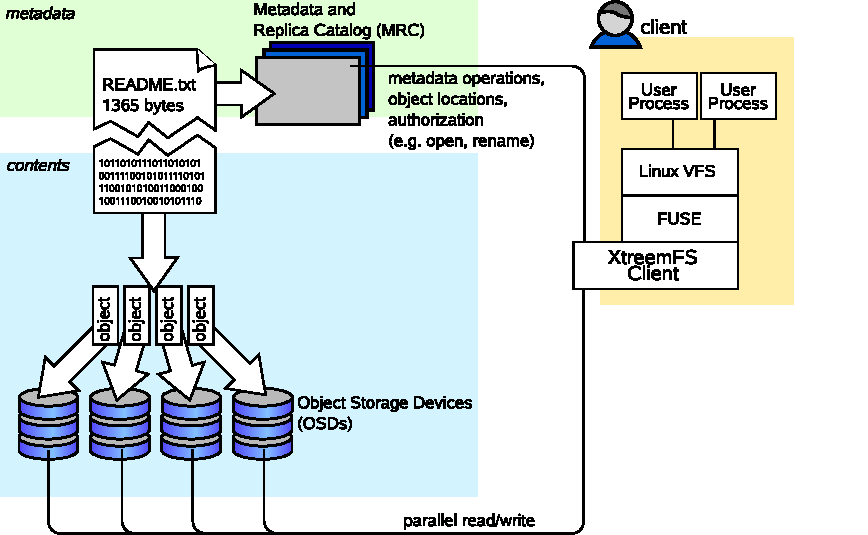
\includegraphics[width=\textwidth]{images/architecture.pdf}
 % architecture.pdf: 417x257 pixel, 72dpi, 14.71x9.07 cm, bb=0 0 417 257
 \caption{The XtreemFS architecture and components.}
 \label{fig:architecture}
\end{figure}


\subsection{The Components of XtreemFS}

An XtreemFS installation contains three types of servers that can run on one or several machines (Fig. \ref{fig:architecture}):

\begin{itemize}
 \item DIR - Directory Service\index{DIR}\index{Directory Service}\\
 The directory service is the central registry for all services in XtreemFS. The MRC uses it to discover storage servers.
 \item MRC - Metadata and Replica Catalog\index{MRC}\index{Metadata Server}\index{Metadata and Replica Catalog}\\
 The MRC stores the directory tree and file metadata such as file name, size or modification time. Moreover, the MRC authenticates users and authorizes access to files.
 \item OSD - Object Storage Device\index{OSD}\index{Storage Server}\index{Object Storage Device}\\
 An OSD stores arbitrary objects of files; clients read and write file data on OSDs.
\end{itemize}

These servers are connected by the \emph{client}\index{Client} to a file system. A client \emph{mounts}\index{Mounting} one of the volumes\index{Volume} of the MRC in a local directory. It translates file system calls into RPCs sent to the respective servers.

The client is implemented as a \emph{FUSE user-level driver} that runs as a normal process. FUSE\index{FUSE} itself is a kernel-userland hybrid that connects the user-land driver to Linux' \emph{Virtual File System (VFS)}\index{VFS} layer where file system drivers usually live.


\subsection{Security}

As usual, XtreemFS security differentiates between authentication and authorization. \emph{Authentication} \index{Authentication} is the process of verifying a user's or client's identity, e.g. validating and reading an X.509 certificate. In contrast, \emph{authorization}\index{Authorization} is the process of checking if a user has the permission to execute a certain operation, e.g. write access to a file.

By default, XtreemFS uses unauthenticated and unencrypted TCP connections. However, \emph{SSL}\index{SSL} can be enabled in all XtreemFS services and the client. Using SSL requires that all users and services provide valid X.509\index{X.509}\index{Certificate} certificates. Any data sent over a SSL connection is encrypted. Using SSL, however, will increase the resource consumption of all components, especially for connection setup (SSL handshake).


\section{Policies}

Many facets of the behavior of XtreemFS can be configured by means of policies. A policy defines how a certain task is performed, e.g.\ how the MRC selects a set of OSDs for a new file, or how it distinguishes between an authorized and an unauthorized user when files are accessed. Various policies have been defined that cover different aspects.

\subsection{OSD Selection Policies} \label{sec:osd_policies}

When a \emph{new file} is created, the MRC must decide which OSDs to use for storing the file content. Based on the required number of OSDs defined in the file's striping policy, an OSD Selection Policy\index{OSD Selection Policy}\index{Policy!OSD Selection Policy} is responsible for selecting the most suitable OSDs. OSD selection policies are assigned at volume granularity. Currently, there are the following policies:

\begin{itemize}
 \item Random OSD Selection (policy id 1)\index{Random OSD Selection}\index{OSD Selection Policy!Random}\\
 Randomly selects OSDs from the list of all available OSDs that are alive and have more than 2GB of free space left.
 \item Proximity-based OSD Selection (policy id 2)\index{Proximity-based OSD Selection}\index{OSD Selection Policy!Proximity-based}\\
 Selects a group of OSDs that are close to each other. The distance is determined by the IP address, i.e. OSDs on the same subnet are preferred. This policy is particularly useful for striping, since it is desirable to have all OSDs at the same site.
 \item DNS based OSD Selection (policy id 3)\index{DNS based OSD Selection}\index{OSD Selection Policy!DNS based}\\
 The FQDN of the client and all OSDs is compared and the maximum match (from the end of the FQDN) is used to sort the OSDs. The policy selects the OSDs with the highest number of characters that match. This policy can be used to automatically select OSDs which are close to the client, if the length of the match between two DNS entries also indicate a low latency between two machines. The minimum match can be modified by setting the xattr '\texttt{xtreemfs.osdsel\_policy\_args}' to an integer value larger 0. OSDs with a match smaller than the minimum match are never used.
\end{itemize}


\subsection{Striping Policies} \label{sec:striping_policies}

XtreemFS allows the content of a file to be distributed among several storage devices (OSDs). This has the benefit, that the file can be read or written in parallel on multiple servers which increases the bandwidth\index{Striping}. The more OSDs are used, the higher the bandwidth available for reading or writing. The number of OSDs is called the striping width\index{Striping!Striping Width}\index{Width, Striping Width}.

A striping policy\index{Striping Policy}\index{Policy!Striping Policy}\index{RAID0} is a rule that defines how the objects are distributed on the available OSDs. Currently, XtreemFS implements only the \texttt{RAID0} policy which simply stores the objects in a round robin fashion on the OSDs. The \texttt{RAID0} policy has two parameters. The striping width\index{Striping Width} defines to how many OSDs the file is distributed. The stripe size\index{Striping!Stripe Size}\index{Stripe Size} defines the size of each object.

When using a striping width of 1, the files are not striped but each file is stored on a single OSD. In that case, you can use any OSD Selection Policy which suits your needs. For striped files (i.e. a striping width larger than 1) we recommend to use the Proximity-based OSD selection policy, because the OSDs onto the files are striped should reside on the same network for better performance and data availability.

Striping over several OSDs enhances the read and write bandwidth of a file, the bandwidth increases the larger the striping width. Please note, that striping also increases the probability of data loss. A striped file will become corrupted even if a single OSDs it is stored on has a disk crash.

\subsection{Authorization - Access Policies} \label{sec:access_policies}

User authorization is managed by means of Access Policies. An access policy defines the access rights for any user on any file or directory contained in a volume. When creating a new volume, the access policy has to be chosen, which cannot be changed in the future. Various access policies can be used: \index{Access Policy}\index{Policy!Access Policy}

\begin{itemize}
 \item Authorize All Policy (policy Id 1)\index{Access Policy!Authorize All}\index{Authorize All Access Policy}\\
No authorization - everyone can do everything. This policy is useful if performance of metadata operations matters more than security, since no recursive evaluation of access policies is done.

 \item POSIX ACLs \& Permissions (policy Id 2)\index{Access Policy!POSIX Permissions}\index{POSIX Permissions Access Policy}\index{Access Policy!POSIX ACLs}\index{POSIX ACLs Access Policy}\\
This access policy implements the traditional POSIX permissions commonly used on Linux, as well as POSIX ACLs, an extension that provides for access control at the granularity of single users and groups. POSIX permissions should be used as the default, as it guarantees maximum compatibility with other file systems.

\item Volume ACLs (policy Id 3)\index{Access Policy!Volume ACLs}\index{Volume ACLs Access Policy}\\
Volume ACLs provide an access control model similar to POSIX ACLs \& Permissions, but only allow one ACL for the whole volume. This means that there is no recursive evaluation of access rights which yields a higher performance at the price of a very coarse-grained access control. 
\end{itemize}


\subsection{Pluggable Policies}

Administrators may extend the set of existing policies by defining \textit{plug-in policies}. Such policies are Java classes that implement a predefined policy interface. Currently, the following policy interfaces exist:

\begin{itemize}
 \item \texttt{org.xtreemfs.common.auth.AuthenticationProvider}\\
   can be used to implement an individual mechanism to authenticate users and groups
 \item \texttt{org.xtreemfs.mrc.ac.FileAccessPolicy}\\
   can be used to implement an individual access control model on files, directories and volumes
 \item \texttt{org.xtreemfs.mrc.osdselection.OSDSelectionPolicy}\\
   can be used to implement an individual policy for allocating OSDs to newly created files
\end{itemize}

Note that there may only be one authentication provider per MRC, while file access policies and OSD selection policies may differ for each volume. The former one is identified by means of its class name (property \texttt{authentication\_provider}, see Sec.\ \ref{sec:config}), while volume-related policies are identified by ID numbers. It is therefore necessary to add a member field

\begin{verbatim}
 public static final long POLICY_ID = 4711;
\end{verbatim}

to all such policy implementations, where \texttt{4711} represents the individual ID number. Administrators have to ensure that such ID numbers neither clash with ID numbers of built-in policies (1-9), nor with ID numbers of other plug-in policies. When creating a new volume, IDs of plug-in policies may be used just like built-in policy IDs.

Plug-in policies have to be deployed in the directory specified by the MRC configuration property \texttt{policy\_dir}. The property is optional; it may be omitted if no plug-in policies are supposed to be used. An implementation of a plug-in policy can be deployed as a Java source or class file located in a directory that corresponds to the package of the class. Library dependencies may be added in the form of source, class or JAR files. JAR files have to be deployed in the top-level directory. All source files in all subdirectories are compiled at MRC start-up time and loaded on demand.


\chapter{XtreemFS Services}

\section{Installation}

When installing XtreemFS, you can choose from two different installation sources: you can download one of the \emph{pre-packaged releases} that we create for most Linux distributions or you can install directly from the \emph{source tarball}. In the pre-packaged release, the server and the client parts are split into separate packages.

\subsection{Prerequisites}

For the pre-packaged release, you will need Sun Java JRE 1.6.0 or newer to be installed on the system.

When building XtreemFS directly from the source, you need a Sun Java JDK 1.6.0 or newer, Ant 1.6.5 or newer and gmake.

\subsection{Installing from Pre-Packaged Releases}

On RPM-based distributions (RedHat, Fedora, SuSE, Mandriva, XtreemOS) you can install the package with


\begin{verbatim}
$> rpm -i xtreemfs-server-1.0.x.rpm
\end{verbatim}


For Debian-based distributions, please use the \texttt{.deb} package provided and install it with


\begin{verbatim}
$> dpkg -i xtreemfs-server-1.0.x.deb
\end{verbatim}


Both packages will also install \texttt{init.d} scripts for an automatic start-up of the services. Use \texttt{insserv xtreemfs-dir}, \texttt{insserv xtreemfs-mrc} and \texttt{insserv xtreemfs-osd}, respectively, to automatically start the services during boot.

\subsection{Installing from Sources}

Extract the tarball with the sources. Change to the top level directory and execute


\begin{verbatim}
$> make server
\end{verbatim}


\section{Configuration}
\label{sec:service_config}

Generally, the configuration files of XtreemFS are located in \texttt{/etc/xos/xtreemfs/} if you installed from packages.


\subsection{A Word about UUIDs}

XtreemFS uses UUIDs\index{UUID} (Universally Unique Identifiers) to be able to identify services and their associated state independently from the machine they are installed on. This implies that you cannot change the \texttt{uuid} of a MRC or OSD after it has been used for the first time!

The Directory Service keeps a mapping from UUID to a port number and IP address or hostname. Currently, each UUID can only be assigned to a single endpoint; the netmask must be ``*'' which means that this mapping is valid in all networks. Upon first start-up, OSDs and MRCs will create the mapping if it does not exist. They will use the first available network device with a public address.

Changing the IP address, hostname or port is possible at any time. Due to the caching of UUIDs in all components it can take some time until the new UUID mapping is used by all OSDs, MRCs and clients. The TTL defines how long an XtreemFS component is allowed to keep entries cached. The default value is 3600 seconds (1 hour). It should be set to shorter durations if services change their IP address frequently.

To create a globally unique UUID you can use tools like \texttt{uuidgen}. During installation the post-install script will automatically create a UUID for each OSD and MRC if it does not have a UUID assigned.

\subsection{Automatic DIR Service Discovery}
\label{sec:autodiscover}
The OSD and MRC discover the DIR service automatically by default. On startup they will broadcast requests to the local LAN and wait up to 10s for a response from a DIR. This works only in a local LAN environment as broadcast messages are not routed to other networks. Local firewalls on the computers on which the services are running can also prevent the automatic discovery from working. The services will select the first DIR which responded which can lead to non-deterministic behaviour if multiple DIR services are present.

\textbf{Security:} The automatic discovery is a potential security risk when used in untrusted environments as any user can start-up DIR services.

A statically configured DIR address and port can be used to disable DIR discovery in the OSD and MRC (see Sec. \ref{sec:config}, \texttt{dir\_service}). By default. the DIR responds to UDP broadcasts. To disable this feature, set  \texttt{discover = false} in the DIR service config file.

\subsection{Authentication}
\label{sec:AuthProvider}
XtreemFS has an interface which allows MRC administrators to choose the way of authenticating users\index{Authentication Provider}. Basically, an MRC has two sources of information on users. The first one is the user id and group ids sent by the client along with each request. In addition, the MRC can use information included in the certificates if SSL is enabled. The Authentication Providers are modules that implement different methods for retrieving the user and group IDs to use.

\subsubsection{UNIX uid/gid - NullAuthProvider}

The NullAuthProvider\index{Authentication Provider!NullAuthProvider}\index{NullAuthProvider} is the default Authentication Provider. It simply uses the user ID and group IDs sent by the XtreemFS client. This means that the client is trusted to send the correct user/group IDs.

The XtreemFS Client will send the user ID and group IDs of the process which executed the file system operation, not of the user who mounted the volume!

The superuser is identified by the user ID \texttt{root} and is allowed to do everything on the MRC. This behavior is similar to NFS with \texttt{no\_root\_squash}.

\subsubsection{Plain SSL Certificates - SimpleX509AuthProvider}

XtreemFS supports two X.509 certificate ``types'' which can be used by the client.\index{Authentication Provider!SimpleX509AuthProvider}\index{SimpleX509AuthProvider} When mounted with a service/host certificate the XtreemFS client is regarded as a trusted system component. The MRC will accept any user ID and groups sent by the client and use them for authorization as with the NullAuthProvider. This setup is useful for volumes which are used by multiple users.

The second certificate type are regular user certificates. The MRC will only accept the user name and group from the certificate and ignore the user ID and groups sent by the client. Such a setup is useful if users are allowed to mount XtreemFS from untrusted machines.

Both certificates are regular X.509 certificates. Service and host certificates are identified by a Common Name (\texttt{CN}) starting with \texttt{host/} or \texttt{xtreemfs-service/}, which can easily be used in existing security infrastructures. All other certificates are assumed to be user certificates.

If a user certificate is used, XtreemFS will take the Distinguished Name (\texttt{DN}) as the user ID and the Organizational Unit (\texttt{OU}) as the group ID.

Superusers must have \texttt{xtreemfs-admin} as part of their Organizational Unit (\texttt{OU}).

\subsubsection{XtreemOS Certificates - XOSAuthProvider}

In contrast to plain X.509 certificates, XtreemOS embeds additional user information as extensions in XtreemOS-User-Certificates.\index{Authentication Provider!XOSAuthProvider}\index{XOSAuthProvider}\index{XtreemOS!XtreemOS Certificates} This authentication provider uses this information (global UID and global GIDs), but the behavior is similar to the SimpleX509AuthProvider.

The superuser is identified by being member of the \texttt{VOAdmin} group.

\subsection{List of Configuration Options}
\label{sec:config}

All configuration parameters that may be used to define the behavior of the different services are listed in this section. Unless marked as optional, a parameter has to occur (exactly once) in a configuration file.

%\makeatletter
%\renewcommand\paragraph{\@startsection{paragraph}{4}{\z@}%
%  {-2.25ex\@plus -1ex \@minus -.2ex}%
%  {1.0ex \@plus .2ex}%
%  {\normalfont\normalsize\bfseries}}
%\makeatother

\subsubsection{\texttt{admin\_password} \textit{optional}}
\begin{tabular}{lp{10cm}}
 Services & DIR, MRC, OSD\\
 Values   & String \\
 Default  & empty\\
 Description & Defines the admin password that must be sent to authorize requests like volume creation, deletion or shutdown.
\end{tabular}

\subsubsection{\texttt{authentication\_provider}}
\begin{tabular}{lp{10cm}}
 Services & MRC\\
 Values   & Java class name \\
 Default  & \texttt{org.xtreemfs.common.auth.NullAuthProvider}\\
 Description & Defines the Authentication Provider to use to retrieve the user identity (user ID and group IDs). See Sec. \ref{sec:AuthProvider} for details.
\end{tabular}

\subsubsection{\texttt{capability\_secret}}
\begin{tabular}{lp{10cm}}
 Services & MRC, OSD\\
 Values   & String \\
 Default  & - \\
 Description & Defines a shared secret between the MRC and all OSDs. The secret is used by the MRC to sign capabilities, i.e. security tokens for data access at OSDs. In turn, an OSD uses the secret to verify that the capability has been issued by the MRC.
\end{tabular}

\subsubsection{\texttt{checksums.enabled}}
\begin{tabular}{lp{10cm}}
 Services & OSD\\
 Values   & true, false \\
 Default  & false \\
 Description & If set to true, the OSD will calculate and store checksums for newly created objects. Each time a checksummed object is read, the checksum will be verified.
\end{tabular}

\subsubsection{\texttt{checksums.algorithm}}
\begin{tabular}{lp{10cm}}
 Services & OSD\\
 Values   & Adler32, CRC32 \\
 Default  & Adler32 \\
 Description & Must be specified if \texttt{checksums.enabled} is enabled. This property defines the algorithm used to create OSD checksums.
\end{tabular}

\subsubsection{\texttt{database.dir}}
\begin{tabular}{lp{10cm}}
 Services & DIR, MRC\\
 Values   & absolute file system path to a directory\\
 Default  & DIR: \texttt{/var/lib/xtreemfs/dir/database},\\
 & MRC: \texttt{/var/lib/xtreemfs/mrc/database}\\
 Description & The directory in which the Directory Service or MRC will store their databases. This directory should never be on the same partition as any OSD data, if both services reside on the same machine. Otherwise, deadlocks may occur if the partition runs out of free disk space!
\end{tabular}

\subsubsection{\texttt{database.log}}
\begin{tabular}{lp{10cm}}
 Services & MRC\\
 Values   & absolute file system path\\
 Default  & MRC: \texttt{/var/lib/xtreemfs/mrc/dblog}\\
 Description & The directory the MRC uses to store database logs. This directory should never be on the same partition as any OSD data, if both services reside on the same machine. Otherwise, deadlocks may occur if the partition runs out of free disk space!
\end{tabular}

\subsubsection{\texttt{debug.level} \textit{optional}}
\begin{tabular}{lp{10cm}}
 Services & DIR, MRC, OSD\\
 Values   & 0, 1, 2, 3, 4, 5, 6, 7 \\
 Default  & 6 \\
 Description & The debug level determines the amount and detail of information written to logfiles. Any debug level includes log messages from lower debug levels. The following log levels exist:
\begin{enumerate}
 \item[0 -] fatal errors
 \item[1 -] alert messages
 \item[2 -] critical errors
 \item[3 -] normal errors
 \item[4 -] warnings
 \item[5 -] notices
 \item[6 -] info messages
 \item[7 -] debug messages
\end{enumerate}
\end{tabular}

\subsubsection{\texttt{debug.categories} \textit{optional}}
\begin{tabular}{lp{10cm}}
 Services & DIR, MRC, OSD\\
 Values   & all, lifecycle, net, auth, stage, proc, db, misc \\
 Default  & all \\
 Description & Debug categories determine the domains for which log messages will be printed. By default, there are no domain restrictions, i.e. log messages form all domains will be included in the log. The following categories can be selected:
\begin{itemize}
 \item[all -] no restrictions on the category
 \item[lifecycle -] service lifecycle-related messages, including startup and shutdown events
 \item[net -] messages pertaining to network traffic and communication between services
 \item[auth -] authentication and authorization-related messages
 \item[stage -] messages pertaining to the flow of requests through the different stages of a service
 \item[proc -] messages about the processing of requests
 \item[db -] messages that are logged in connection with database accesses
 \item[misc -] any other log messages that do not fit in one of the previous categories
\end{itemize}
Note that it is possible to specify multiple categories by means of a comma or space-separated list.
\end{tabular}

\subsubsection{\texttt{dir\_service.host}}
\begin{tabular}{lp{10cm}}
 Services & MRC, OSD\\
 Values   & hostname or IP address \\
 Default  & .autodiscover \\
 Description & Specifies the hostname or IP address of the directory service (DIR) at which the MRC or OSD should register. The MRC also uses this directory service to find OSDs. If set to \texttt{.autodiscover} the service will use the automatic DIR discovery mechanism (see Sec. \ref{sec:autodiscover}).
\end{tabular}

\subsubsection{\texttt{dir\_service.port}}
\begin{tabular}{lp{10cm}}
 Services & MRC, OSD\\
 Values   & 1 .. 65535 \\
 Default  & 32638 \\
 Description & Specifies the port on which the remote directory service is listening. Must be identical to the \texttt{listen\_port} in your directory service configuration.
\end{tabular}

\subsubsection{\texttt{discover} \textit{optional}}
\begin{tabular}{lp{10cm}}
 Services & DIR\\
 Values   & true, false \\
 Default  & true \\
 Description & If set to true the DIR will received UDP broadcasts and advertise itself in response to XtreemFS components using the DIR automatic discoery mechanism. If set to false, the DIR will ignore all UDP traffic. For details see Sec. \ref{sec:autodiscover}.
\end{tabular}

\subsubsection{\texttt{geographic\_coordinates}}
\begin{tabular}{lp{10cm}}
 Services & DIR, MRC, OSD\\
 Values   & String \\
 Default  & empty \\
 Description & Specifies the geographic coordinates which are registered with the directory service. Used e.g. by the web console.
\end{tabular}

\subsubsection{\texttt{http\_port}}
\begin{tabular}{lp{10cm}}
 Services & DIR, MRC, OSD\\
 Values   & 1 .. 65535 \\
 Default  & 30636 (MRC), 30638 (DIR), 30640 (OSD)\\
 Description & Specifies the geographic coordinates which are registered with the directory service. Used e.g. by the web console.
\end{tabular}

\subsubsection{\texttt{listen.address} \textit{optional}}
\begin{tabular}{lp{10cm}}
 Services & OSD\\
 Values   & IP address \\
 Default  & -\\
 Description & If specified, defines the interface to listen on. If not specified, the service will listen on all interfaces (any).
\end{tabular}

\subsubsection{\texttt{listen.port}}
\begin{tabular}{lp{10cm}}
 Services & DIR, MRC, OSD\\
 Values   & 1 .. 65535 \\
 Default  & DIR: 32638,\\
 & MRC: 32636,\\
 & OSD: 32640 \\
 Description & The port to listen on for incoming connections (TCP). The OSD uses TCP and UDP on the specified port. Make sure to configure your firewall to allow incoming TCP and UDP traffic on the specified port.
\end{tabular}

\subsubsection{\texttt{local\_clock\_renewal}}
\begin{tabular}{lp{10cm}}
 Services & MRC, OSD\\
 Values   & milliseconds \\
 Default  & 50\\
 Description & Reading the system clock is a slow operation on some systems (e.g. Linux) as it is a system call. To increase performance, XtreemFS services use a local variable which is only updated every \texttt{local\_clock\_renewal} milliseconds.
\end{tabular}

\subsubsection{\texttt{no\_atime}}
\begin{tabular}{lp{10cm}}
 Services & MRC\\
 Values   & true, false \\
 Default  & true\\
 Description & The POSIX standard defines that the atime (timestamp of last file access) is updated each time a file is opened, even for read. This means that there is a write to the database and hard disk on the MRC each time a file is read. To reduce the load, many file systems (e.g. ext3) including XtreemFS can be configured to skip those updates for performance. It is strongly suggested to disable atime updates by setting this parameter to true.
\end{tabular}

\subsubsection{\texttt{no\_fsync} \textit{optional}}
\begin{tabular}{lp{10cm}}
 Services & MRC\\
 Values   & true, false \\
 Default  & false\\
 Description & By default, the MRC will write all file-modifying operations (such as create file, delete etc.) to disk followed by a \texttt{fsync} to ensure data is written to the hard disk. While this ensures maximum data safety in case of crash of the MRC server, it also reduces the performance of the MRC. Set this to true, if you want much higher performance at the risk of losing some recent file operations in case of a server crash.
\end{tabular}

\subsubsection{\texttt{object\_dir}}
\begin{tabular}{lp{10cm}}
 Services & OSD\\
 Values   & absolute file system path to a directory\\
 Default  & \texttt{/var/lib/xtreemfs/osd/}\\
 Description & The directory in which the OSD stores the objects. This directory should never be on the same partition as any DIR or MRC database, if both services reside on the same machine. Otherwise, deadlocks may occur if the partition runs out of free disk space!
\end{tabular}

\subsubsection{\texttt{osd\_check\_interval}}
\begin{tabular}{lp{10cm}}
 Services & MRC\\
 Values   & seconds \\
 Default  & 300\\
 Description & The MRC regularly asks the directory service for suitable OSDs to store files on (see OSD Selection Policy, Sec. \ref{sec:osd_policies}). This parameter defines the interval between two updates of the list of suitable OSDs.
\end{tabular}

\subsubsection{\texttt{remote\_time\_sync}}
\begin{tabular}{lp{10cm}}
 Services & MRC, OSD\\
 Values   & milliseconds \\
 Default  & 30,000\\
 Description & MRCs and OSDs all synchronize their clocks with the directory service to ensure a loose clock synchronization of all services. This is required for leases to work correctly. This parameter defines the interval in milliseconds between time updates from the directory service.
\end{tabular}

\subsubsection{\texttt{report\_free\_space}}
\begin{tabular}{lp{10cm}}
 Services & OSD\\
 Values   & true, false\\
 Default  & true\\
 Description & If set to true, the OSD will report its free space to the directory service. Otherwise, it will report zero, which will cause the OSD not to be used by the OSD Selection Policies (see Sec. \ref{sec:osd_policies}).
\end{tabular}

\subsubsection{\texttt{ssl.enabled}}
\begin{tabular}{lp{10cm}}
 Services & DIR, MRC, OSD\\
 Values   & true, false \\
 Default  & false \\
 Description & If set to true, the service will use SSL to authenticate and encrypt connections. The service will not accept non-SSL connections if \texttt{ssl.enabled} is set to true.
\end{tabular}

\subsubsection{\texttt{ssl.service\_creds}}
\begin{tabular}{lp{10cm}}
 Services & DIR, MRC, OSD\\
 Values   & path to file\\
 Default  & DIR: \texttt{/etc/xos/xtreemfs/truststore/certs/ds.p12}, \\
 & MRC: \texttt{/etc/xos/xtreemfs/truststore/certs/mrc.p12}, \\
 & OSD: \texttt{/etc/xos/xtreemfs/truststore/certs/osd.p12}\\
 Description & Must be specified if \texttt{ssl.enabled} is enabled. Specifies the file containing the service credentials (X.509 certificate and private key). PKCS\#12 and JKS format can be used, set \texttt{ssl.service\_creds.container} accordingly. This file is used during the SSL handshake to authenticate the service.
\end{tabular}

\subsubsection{\texttt{ssl.service\_creds.container}}
\begin{tabular}{lp{10cm}}
 Services & DIR, MRC, OSD\\
 Values   & \texttt{pkcs12} or \texttt{JKS}\\
 Default  & \texttt{pkcs12}\\
 Description & Must be specified if \texttt{ssl.enabled} is enabled. Specifies the file format of the \texttt{ssl.service\_creds} file.
\end{tabular}

\subsubsection{\texttt{ssl.service\_creds.pw}}
\begin{tabular}{lp{10cm}}
 Services & DIR, MRC, OSD\\
 Values   & String\\
 Default  & -\\
 Description & Must be specified if \texttt{ssl.enabled} is enabled. Specifies the password which protects the credentials file \texttt{ssl.service\_creds}.
\end{tabular}

\subsubsection{\texttt{ssl.trusted\_certs}}
\begin{tabular}{lp{10cm}}
 Services & DIR, MRC, OSD\\
 Values   & path to file\\
 Default  & \texttt{/etc/xos/xtreemfs/truststore/certs/xosrootca.jks}\\
 Description & Must be specified if \texttt{ssl.enabled} is enabled. Specifies the file containing the trusted root certificates (e.g. CA certificates) used to authenticate clients.
\end{tabular}

\subsubsection{\texttt{ssl.trusted\_certs.container}}
\begin{tabular}{lp{10cm}}
 Services & DIR, MRC, OSD\\
 Values   & \texttt{pkcs12} or \texttt{JKS}\\
 Default  & \texttt{JKS}\\
 Description & Must be specified if \texttt{ssl.enabled} is enabled. Specifies the file format of the \texttt{ssl.trusted\_certs} file.
\end{tabular}

\subsubsection{\texttt{ssl.trusted\_certs.pw}}
\begin{tabular}{lp{10cm}}
 Services & DIR, MRC, OSD\\
 Values   & String\\
 Default  & -\\
 Description & Must be specified if \texttt{ssl.enabled} is enabled. Specifies the password which protects the trusted certificates file \texttt{ssl.trusted\_certs}.
\end{tabular}


\subsubsection{\texttt{uuid}}
\begin{tabular}{lp{10cm}}
 Services & MRC, OSD\\
 Values   & String, but limited to alphanumeric characters, - and . \\
 Default  & - \\
 Description & Must be set to a unique identifier, preferably a UUID according to RFC 4122. UUIDs can be generated with \texttt{uuidgen}. Example: \texttt{eacb6bab-f444-4ebf-a06a-3f72d7465e40}.
\end{tabular}




\subsection{Configuring SSL Support}

In order to enable certificate-based authentication in an XtreemFS installation, services need to be equipped with X.509\index{X.509}\index{Certificate}\index{Credentials} certificates. Certificates are used to establish a mutual trust relationship among XtreemFS services and between the XtreemFS client and XtreemFS services.

It is not possible to mix SSL-enabled and non-SSL services in an XtreemFS installation!

Each XtreemFS service needs a certificate and a private key in order to be run. Once they have been created and signed, the credentials may need to be converted into the correct file format. XtreemFS services also need a \textit{trust store} that contains all trusted Certification Authority certificates.

By default, certificates and credentials for XtreemFS services are stored in
\begin{verbatim}
/etc/xos/xtreemfs/truststore/certs
\end{verbatim}


\subsubsection{Converting PEM files to PKCS\#12}
The simplest way to provide the credentials to the services is by converting your signed certificate and private key into a PKCS\#12\index{PKCS\#12} file using \texttt{openssl}:


\begin{verbatim}
$> openssl pkcs12 -export -in ds.pem -inkey ds.key \
   -out ds.p12 -name "DS"
$> openssl pkcs12 -export -in mrc.pem -inkey mrc.key \
   -out mrc.p12 -name "MRC"
$> openssl pkcs12 -export -in osd.pem -inkey osd.key \
   -out osd.p12 -name "OSD"
\end{verbatim}


This will create three PKCS12 files (\texttt{ds.p12}, \texttt{mrc.p12} and \texttt{osd.p12}), each containing the private key and certificate for the respective service. The passwords chosen when asked must be set as a property in the corresponding service configuration file.



\subsubsection{Importing trusted certificates from PEM into a JKS}

The certificate (or multiple certificates) from your CA (or CAs) can be imported into a Java Keystore (JKS) \index{JKS}\index{Java KeyStore} using the Java keytool which comes with the Java JDK or JRE.

Execute the following steps for each CA certificate using the same keystore file.


\begin{verbatim}
$> keytool -import -alias rootca -keystore trusted.jks \
   -trustcacerts -file ca-cert.pem
\end{verbatim}


This will create a new Java Keystore \texttt{trusted.jks} with the CA certificate in the current working directory. The password chosen when asked must be set as a property in the service configuration files.

Note: If you get the following error
\begin{verbatim}
$> keytool error: java.lang.Exception: Input not an X.509 certificate
\end{verbatim}
you should remove any text from the beginning of the certificate (until the \texttt{-----BEGIN CERTIFICATE-----} line).


\subsubsection{Sample Setup}

Users can easily set up their own CA (certificate authority)\index{Certificate Authority}\index{CA!Certificate Authority} and create and sign certificates using \texttt{openssl} for a test setup.

\begin{enumerate}
 \item Set up your test CA.
	\begin{enumerate}
	\item Create a directory for your CA files
		\begin{verbatim}
		$> mkdir ca
		\end{verbatim}

	\item Create a private key and certificate request for your CA.
		\begin{verbatim}
		$> openssl req -new -newkey rsa:1024 -nodes -out ca/ca.csr \
		   -keyout ca/ca.key
		\end{verbatim}

		Enter something like XtreemFS-DEMO-CA as the common name (or something else, but make sure the name is different from the server and client name!).
	\item Create a self-signed certificate for your CA which is valid for one year.
		\begin{verbatim}
		$> openssl x509 -trustout -signkey ca/ca.key -days 365 -req \
		   -in ca/ca.csr -out ca/ca.pem
		\end{verbatim}

	\item Create a file with the CA's serial number
		\begin{verbatim}
		$> echo "02" > ca/ca.srl
		\end{verbatim}

 \end{enumerate}
 \item Set up the certificates for the services and the XtreemFS Client.\\
	Replace \texttt{\textit{service}} with \texttt{dir}, \texttt{mrc}, \texttt{osd} and \texttt{client}.
	\begin{enumerate}
	\item Create a private key for the service.\\
	      Use \texttt{XtreemFS-DEMO-\textit{service}} as the common name for the certificate.
		\begin{Verbatim}[commandchars=\\\{\}]
$> openssl req -new -newkey rsa:1024 -nodes \
   -out \textit{service}.req \
   -keyout \textit{service}.key
		\end{Verbatim}

	\item Sign the certificate with your demo CA.\\
		The certificate is valid for one year.
		\begin{Verbatim}[commandchars=\\\{\}]
$> openssl x509 -CA ca/ca.pem -CAkey ca/ca.key \
   -CAserial ca/ca.srl -req \
   -in \textit{service}.req \
   -out \textit{service}.pem -days 365
		\end{Verbatim}

	\item Export the service credentials (certificate and private key) as a PKCS\#12 file.\\
		Use ``passphrase'' as export password. You can leave the export password empty for the XtreemFS Client to avoid being asked for the password on mount.
		\begin{Verbatim}[commandchars=\\\{\}]
$> openssl pkcs12 -export -in \textit{service}.pem -inkey \
   \textit{service}.key \
   -out \textit{service}.p12 -name "\textit{service}"
		\end{Verbatim}

	\item Copy the PKCS\#12 file to the certificates directory.
		\begin{Verbatim}[commandchars=\\\{\}]
	$> mkdir -p /etc/xos/xtreemfs/truststore/certs
    $> cp \textit{service}.p12 /etc/xos/xtreemfs/truststore/certs
		\end{Verbatim}

	\end{enumerate}
 \item Export your CA's certificate to the trust store and copy it to the certificate dir.\\
	You should answer ``yes'' when asked ``Trust this certificate''.\\
	Use ``passphrase'' as passphrase for the keystore.
	\begin{verbatim}
	$> keytool -import -alias ca -keystore trusted.jks\
	   -trustcacerts -file ca/ca.pem
	$> cp  trusted.jks /etc/xos/xtreemfs/truststore/certs
	\end{verbatim}

 \item Configure the services.
	Edit the configuration file for all your services. Set the following configuration options (see Sec. \ref{sec:service_config} for details).\\
	\texttt{ssl.enabled = true}\\
	\texttt{ssl.service\_creds.pw = passphrase}\\
	\texttt{ssl.service\_creds.container = pkcs12}\\
	\texttt{ssl.service\_creds = /etc/xos/xtreemfs/truststore/certs/\textit{service}.p12}\\
	\texttt{ssl.trusted\_certs = /etc/xos/xtreemfs/truststore/certs/trusted.jks}\\
	\texttt{ssl.trusted\_certs.pw = passphrase}\\
	\texttt{ssl.trusted\_certs.container = jks}
 \item Start up the XtreemFS services (see Sec. \ref{sec:startstopservice}).
 \item Create a new volume (see Sec. \ref{sec:create_volume} for details).
	\begin{verbatim}
	$> xtfs_mkvol --pkcs12-file-path=\
	   /etc/xos/xtreemfs/truststore/certs/client.p12 localhost/test
	\end{verbatim}

 \item Mount the volume (see Sec. \ref{sec:mount_vol} for details).
	\begin{verbatim}
	$> xtfs_mount --pkcs12-file-path=\
	   /etc/xos/xtreemfs/truststore/certs/client.p12 localhost/test /mnt
	\end{verbatim}

\end{enumerate}


\section{Management}
This section covers all tools and functionality for XtreemFS management and tracing. In general, the use of management tools is restricted to superusers.

\subsection{Starting and Stopping the XtreemFS services}
\label{sec:startstopservice}

If you installed a \emph{pre-packaged release} you can start, stop and restart the services with the \texttt{init.d}\index{init.d} scripts:
	\begin{verbatim}
	$> /etc/init.d/xtreemfs-ds start
	$> /etc/init.d/xtreemfs-mrc start
	$> /etc/init.d/xtreemfs-osd start
	\end{verbatim}
or
	\begin{verbatim}
	$> /etc/init.d/xtreemfs-ds stop
	$> /etc/init.d/xtreemfs-mrc stop
	$> /etc/init.d/xtreemfs-osd stop
	\end{verbatim}


\textbf{Note} that the Directory Service should be started first, in order to allow other services an immediate registration. Once a Directory Service and at least one OSD and MRC are running, XtreemFS is operational.

\subsection{Web-based Status Page}

The XtreemFS services all have a HTML status page\index{Status Page} which can be used to check if the service is working correctly (Fig. \ref{fig:screenshot_status}). It can be displayed by opening the service URL in your favorite web browser, e.g.\\ \texttt{http://my-mrc-host.com:30636/}. Make sure to use the right port, see \texttt{http\_port} in the service config file.

\begin{figure}[h]
 \centering
 \resizebox{0.7\linewidth}{!}{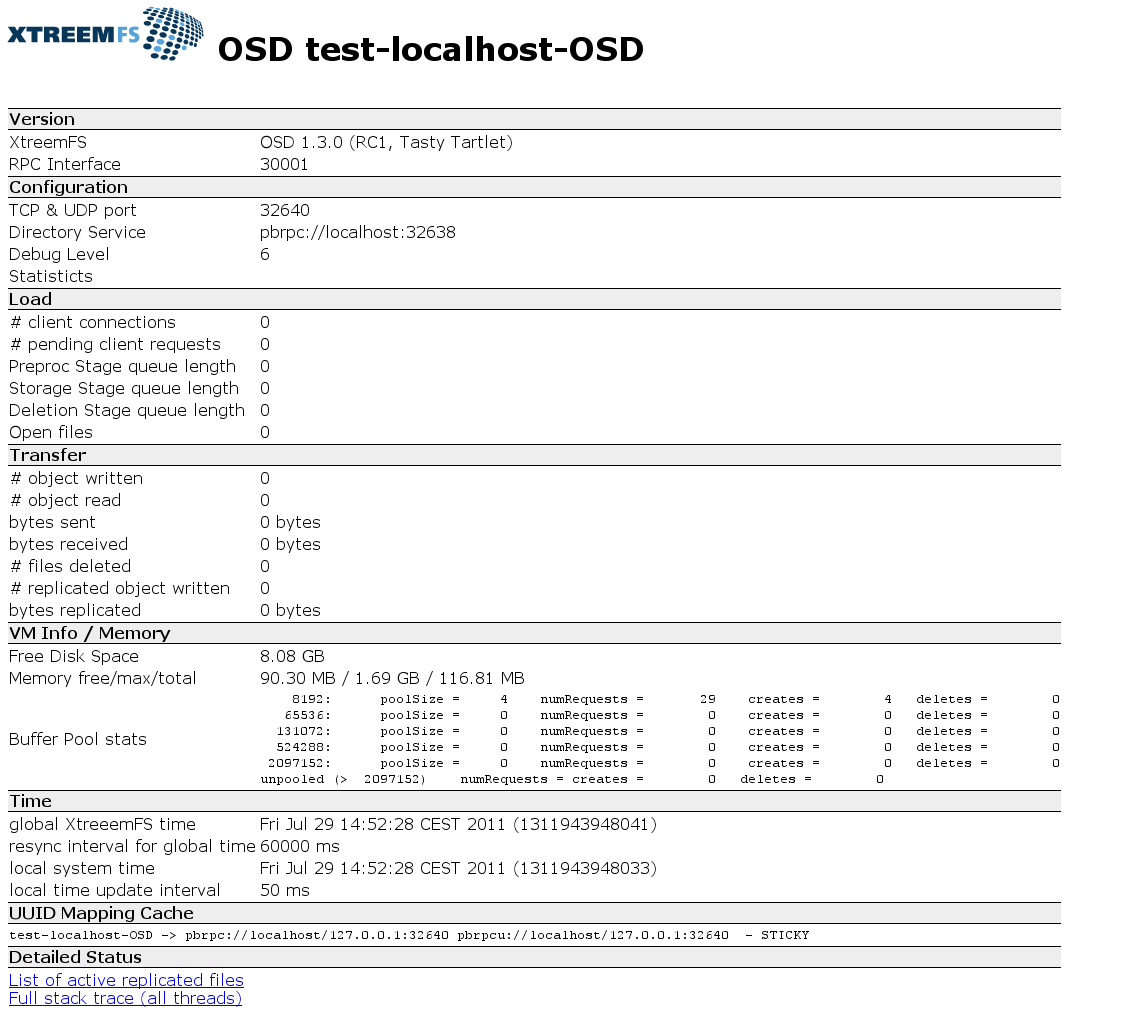
\includegraphics{images/screenshot_status.png}}
 % screenshot_status.png: 817x847 pixel, 72dpi, 28.82x29.88 cm, bb=0 0 817 847
 \caption{OSD status web page}
 \label{fig:screenshot_status}
\end{figure}


\subsection{Creating Volumes}
\label{sec:create_volume}

Volumes can be created with the \texttt{xtfs\_mkvol} command line utility. Please see \texttt{man xtfs\_mkvol} for a full list of options and usage\index{Create Volume}\index{Volume!Create}\index{xtfs\_mkvol}.

When creating a volume, it is recommended to specify the access policy (see Sec. \ref{sec:access_policies}). If not specified, POSIX permissions/ACLs will be chosen by default. Access policies cannot be changed afterwards.

An OSD selection policy (see Sec. \ref{sec:osd_policies}) can also be specified per volume, but can be changed anytime. By default, a random selection of available OSDs is assigned to newly created files.

In addition, it is recommended to set a default striping policy (see Sec. \ref{sec:striping_policies}). If no per-file or per-directory default striping policy overrides the volume's default striping policy, the volume's policy is used for new files and directories. If no volume policy is explicitly defined, a RAID0 policy with a stripe size of 128kB and a width of 1 will be assigned to the volume.

An example call to \texttt{xtfs\_mkvol} for creating a volume with POSIX ACLs, 256kB stripe size and a stripe width of 1 (which means no striping):


\begin{verbatim}
$> xtfs_mkvol -a POSIX -p RAID0 -s 256 -w 1 \
   my-mrc-host.com:32636/myVolume
\end{verbatim}

\subsection{Deleting Volumes}

The \texttt{xtfs\_rmvol} tool can be used to delete a volume. This also \emph{deletes all files and data on that volume}! Please see \texttt{man xtfs\_rmvol} for a full list of options and usage\index{Delete Volume}\index{Volume!Delete}\index{xtfs\_rmvol}.

Example call to \texttt{xtfs\_rmvol} to delete \texttt{myVolume}:


\begin{verbatim}
$> xtfs_rmvol my-mrc-host.com:32636/myVolume
\end{verbatim}

Volume deletion is restricted to volume owners and superusers.

\subsection{MRC Database Conversion}

The format in which the MRC stores its data on disk may change with future XtreemFS versions. In order that XtreemFS server components may be updated without losing the whole content of the file system, it is possible to create a version-independent XML representation of the metadata stored in MRC database.

Such an XML representation can e.g.\ be created as follows:

\begin{verbatim}
$> xtfs_mrcdbtool -mrc my-mrc-host.com:32636 \
   dump /tmp/dump.xml
\end{verbatim}

This call will create a file \texttt{dump.xml} containing the entire MRC database content in the \texttt{/tmp} directory at \texttt{my-mrc-host.com}.

To restore an MRC database from a dump, execute

\begin{verbatim}
$> xtfs_mrcdbtool -mrc my-mrc-host.com:32636 \
   restore /tmp/dump.xml
\end{verbatim}

This will restore the database stored in \texttt{/tmp/dump.xml} at \texttt{my-mrc-host.com}. Note that for safety reasons, it is only possible to restore a database from a dump if the database of the running MRC does not have any content. To restore an MRC database, it is thus necessary to delete all MRC database files before starting the MRC.

\subsection{Scrubbing and Cleanup}

In real-world environments, errors occur in the course of creating, modifying or deleting files. This can cause corruptions of file data or metadata. Such things happen e.g.\ if the client is suddenly terminated, or loses connection with a server component. There are several such scenarios: if a client writes to a file but does not report file sizes received from the OSD back to the MRC, inconsistencies between the file size stored in the MRC and the actual size of all objects in the OSD will occur. If a client deletes a file from the directory tree, but cannot reach the OSD, orphaned objects will remain on the OSD. If an OSD is terminated during an ongoing write operation, file content will become corrupted.

In order to detect and, if possible, resolve such inconsistencies, tools for scrubbing and OSD cleanup exist. To check the consistency of file sizes and checksums, the following command can be executed:

\begin{verbatim}
$> xtfs_scrub -dir oncrpc://my-dir-host.com:32638 xtreemfsVolume
\end{verbatim}

This will scrub each file in the volume \texttt{myVolume}, i.e.\ check file size consistency and set the correct file size on the MRC, if necessary, and check whether an invalid checksum in the OSD indicates a corrupted file content. The \texttt{-dir} argument specifies the directory service that will be used to resolve service UUIDs. Please see \texttt{man xtfs\_scrub} for further details.

A second tool scans an OSD for orphaned objects, which can be used as follows:

\begin{verbatim}
$> xtfs_cleanup -dir oncrpc://localhost:32638 \
   uuid:u2i3-28isu2-iwuv29-isjd83
\end{verbatim}
The given UUID identifies the OSD to clean and will be resolved by the
directory service defined by the \texttt{-dir} option (localhost:32638 in this example).
The process will be started and can be stopped by setting the option
\texttt{-stop}. To watch the cleanup progress use option \texttt{-i} for the
interactive mode. For further informations see \texttt{man xtfs\_cleanup}.


\chapter{The XtreemFS Client}

\section{Installation}

As for the XtreemFS Services, there are two different installation sources for the XtreemFS Client: \emph{pre-packaged releases} and \emph{source tarballs}.

\subsection{Prerequisites}

For both installations you need FUSE 2.6 or newer, openSSL 0.9.8 or newer and a Linux 2.6 kernel. For optimal performance we suggest to use FUSE 2.8 with a kernel version 2.6.26 or newer.

To build the XtreemFS Client from sources, you need the openSSL headers (e.g. openssl-devel package), python $\geq$ 2.4, and gcc-c++ $\geq$ 4.2.

\subsection{Installing from Pre-Packaged Releases}

On RPM-based distributions (RedHat, Fedora, SuSE, Mandriva, XtreemOS) you can install the package with


\begin{verbatim}
$> rpm -i xtreemfs-client-1.0.x.rpm
\end{verbatim}


For Debian-based distributions, please use the \texttt{.deb} package provided and install it with


\begin{verbatim}
$> dpkg -i xtreemfs-client-1.0.x.deb
\end{verbatim}



\subsection{Installing from Sources}

Extract the tarball with the sources. Change to the top level directory and execute


\begin{verbatim}
$> make client
\end{verbatim}


\section{Mounting and Un-mounting}
\label{sec:mount_vol}

Before mounting XtreemFS volumes, please ensure that the FUSE kernel module is loaded.\index{Volume!Mount}\index{Mount}\index{xtfs\_mount} Please check your distribution's manual to see, if users must be in a special group (e.g. \texttt{trusted} in openSUSE) to be allowed to mount FUSE.


\begin{verbatim}
$> su
Password:
#> modprobe fuse
#> exit
\end{verbatim}


To mount an XtreemFS volume use the \texttt{xtfs\_mount} tool.


\begin{verbatim}
$> xtfs_mount remote.dir.machine/myVolume /xtreemfs
\end{verbatim}


\texttt{remote.dir.machine} describes the host with the Directory Service at which the volume is registered; \texttt{myVolume} is the name of the volume name to be mounted. \texttt{/xtreemfs} is the directory on the local file system to which the XtreemFS volume will be mounted. For more options, please refer to \texttt{man xtfs\_mount}.

The client will immediately go into background and won't display any error messages. Use the \texttt{-f} option to prevent the mount process from going into background and get all error messages printed to the console.

Access to a FUSE mount is usually restricted to the user who mounted the volume. To allow the root user or any other user on the system to access the mounted volume, the FUSE options \texttt{-o allow\_root} and \texttt{-o allow\_other} can be used with \texttt{xtfs\_mount}. They are, however, mutually exclusive. In order to use these options, the system administrator must create a FUSE configuration file \texttt{/etc/fuse.conf} and add a line\index{allow\_others option}\index{allow\_root option}\index{user\_allow\_other option} \texttt{user\_allow\_other}.

To check that a volume is mounted use the \texttt{mount} command. It ouputs a list of all mounts in the system. XtreemFS volumes are listed as \texttt{type fuse}:

\begin{verbatim}
/dev/fuse on /xtreemfs type fuse (rw,nosuid,nodev,user=userA)
\end{verbatim}

Volumes are unmounted using the \texttt{xtfs\_umount} tool\index{Volume!Un-mount}\index{Unmount}\index{xtfs\_umount}.


\begin{verbatim}
$> xtfs_umount /xtreemfs
\end{verbatim}



\section{Reading XtreemFS-specific File Info}

In addition to the regular file system information provided by the \texttt{stat} Linux utility, XtreemFS provides the \texttt{xtfs\_stat}\index{xtfs\_stat}\index{XtreemFS stat} tool which displays XtreemFS specific information for a file or directory.


\begin{verbatim}
$> cd /xtreemfs
$> echo 'Hello World' > test.txt
$> xtfs_stat remote.mrc.machine/myVolume/test.txt
\end{verbatim}


will produce output similar to the following:


\begin{verbatim}
-----
  type           = directory
  nlink          = 1
  size           = 0
  atime          = 2009-05-05T09:44:16.000Z
  mtime          = 2009-05-05T10:10:06.000Z
  ctime          = 2009-05-05T10:10:06.000Z
  owner user id  = xtreemfs
  owner group id = users
  file_id        = 0fa6c684-4885-48b1-a678-babdfae8db37:1
  truncate epoch = 2031654
\end{verbatim}


The fileID \index{fileID} is the unique identifier of the file used on the OSDs to identify the file's objects. The owner/group fields are shown as reported by the MRC, you may see other names on your local system if there is no mapping (i.e. the file owner does not exist as a user on your local machine).
Finally, the XtreemFS replica list shows the striping policy of the file, the number of replicas and for each replica, the OSDs used to store the objects.


\section{Changing Striping Policies}

It is not (yet) possible to change the striping policy of an existing file, as this would require moving and reformatting data among OSDs. However, individual striping policies can be assigned to new files (i.e. empty files) by changing the default striping policy of the parent directory or volume. For this purpose, XtreemFS provides the \texttt{xtfs\_sp}\index{xtfs\_sp}\index{XtreemFS striping policy tool} tool. The tool can be used to change the striping policy that will be assigned to newly created files.

\begin{verbatim}
$> xtfs_sp --set -p RAID0 -w 4 -s 256 /xtreemfs
\end{verbatim}

In addition, the tool can be used to retrieve the default striping policy of a volume or directory.

\begin{verbatim}
$> xtfs_sp --get /xtreemfs
\end{verbatim}

The output will be similar to the following:

\begin{verbatim}
file:         /xtreemfs
policy:       STRIPING_POLICY_RAID0
stripe-size:  4
width (kB):   256
\end{verbatim}

When creating a new file, XtreemFS will first check whether a default striping policy has been assigned to the parent directory. If this is not the case, the default striping policy for the volume will be used as the striping policy for the new file. Changing a volume's or directory's default striping policy requires superuser access rights or ownership of the directory or volume.

\chapter{Troubleshooting and Support}

\section{Logfiles}

The logfiles for the XtreemFS services are located in \texttt{/var/log/xtreemfs}. The client generates no output, unless the \texttt{-f} and \texttt{-d INFO} options are specified.

\section{Support}
Please visit the \href{http://www.XtreemFS.org}{XtreemFS website at www.XtreemFS.org} for links to the user mailing list and IRC channel.

\section{Troubleshooting}

\textbf{Problem: }The client hangs when opening/copying/creating a file but operations like \texttt{ls} or \texttt{mkdir} work.

\textbf{Solution: }This problem can occurr when an OSD uses a UUID which resolves to an address that the client cannot (correctly) resolve. If you use e.g. \texttt{localhost:32640} as the UUID for the OSD, the client will try to contact the local machine instead of the machine on which the OSD runs. Check the status page of your Directory Service and check the UUID of the OSDs.

\textbf{Problem: } \texttt{xtfs\_mount} does not print an error message but the volume is not mounted (i.e. not listed in the output of \texttt{mount}).

\textbf{Solution: } The client \texttt{xtfs\_mount} automatically goes into background and does not print any error messages or warinings. Use the \texttt{-f} flag when mounting to prevent the client from going into background. All error messages will be printed to the console.

\appendix

\chapter{XtreemOS Integration}

\subsubsection{XtreemFS Security Preparations}
\label{installconf-xfs-security}

XtreemFS\index{XtreemOS!Integration} can be integrated in an existing XtreemOS VO security infrastructure. XtreemOS uses X.509 certificates to authenticate users in a Grid system, so the general setup is similar to a normal SSL-based configuration.

Thus, in an XtreemOS environment, certificates have to be created for the services as a first step. This is done by issuing a \textit{Certificate Signing Request (CSR)} to the RCA server by means of the \texttt{create-server-csr} command. For further details, see the Section Using the RCA in the XtreemOS User Guide.

Signed certificates and keys generated by are RCA infrastructure are stored locally in PEM format. Since XtreemFS services are currently not capable of processing PEM certificates, keys and certificates have to be converted to PKCS12 and Java Keystore format, respectively.

Each XtreemFS service needs a certificate and a private key in order to be run. Once they have created and signed, the conversion has to take place. Assuming that certificate/private key pairs reside in the current working directory for the Directory Service, an MRC and an OSD (\texttt{ds.pem}, \texttt{ds.key}, \texttt{mrc.pem}, \texttt{mrc.key}, \texttt{osd.pem} and \texttt{osd.key}), the conversion can be initiated with the following commands:


\begin{verbatim}
$> openssl pkcs12 -export -in ds.pem -inkey ds.key \
   -out ds.p12 -name "DS"
$> openssl pkcs12 -export -in mrc.pem -inkey mrc.key \
   -out mrc.p12 -name "MRC"
$> openssl pkcs12 -export -in osd.pem -inkey osd.key \
   -out osd.p12 -name "OSD"
\end{verbatim}

This will create three PKCS12 files (\texttt{ds.p12}, \texttt{mrc.p12} and \texttt{osd.p12}), each containing the private key and certificate for the respective service.

XtreemFS services need a \textit{trust store} that contains all trusted Certification Authority certificates. Since all certificates created via the RCA have been signed by the XtreemOS CA, the XtreemOS CA certificate has to be included in the trust store. To create a new trust store containing the XtreemOS CA certificate, execute the following command:


\begin{verbatim}
$> keytool -import -alias xosrootca -keystore xosrootca.jks \
   -trustcacerts -file \
   /etc/xos/truststore/xtreemosrootcacert.pem
\end{verbatim}

This will create a new Java Keystore \texttt{xosrootca.jks} with the XtreemOS CA certificate in the current working directory. The password chosen when asked will later have to be added as a property in the service configuration files.

Once all keys and certificates have been converted, the resulting files should be moved to \texttt{/etc/xos/xtreemfs/truststore/certs} as root:


\begin{verbatim}
# mv ds.p12 /etc/xos/xtreemfs/truststore/certs
# mv mrc.p12 /etc/xos/xtreemfs/truststore/certs
# mv osd.p12 /etc/xos/xtreemfs/truststore/certs
# mv xosrootca.jks /etc/xos/xtreemfs/truststore/certs
\end{verbatim}


For setting up a \textit{secured} XtreemFS infrastructure, each service provides the following properties:


\begin{verbatim}
# specify whether SSL is required
ssl.enabled = true

# server credentials for SSL handshakes
ssl.service_creds = /etc/xos/xtreemfs/truststore/certs/\
service.p12
ssl.service_creds.pw = xtreemfs
ssl.service_creds.container = pkcs12

# trusted certificates for SSL handshakes
ssl.trusted_certs = /etc/xos/xtreemfs/truststore/certs/\
xosrootca.jks
ssl.trusted_certs.pw = xtreemfs
ssl.trusted_certs.container = jks
\end{verbatim}

\texttt{service.p12} refers to the converted file containing the credentials of the respective service. Make sure that all paths and passphrases (\texttt{xtreemfs} in this example) are correct.



\chapter{Command Line Utilities}

\begin{description}
 \item[xtfs\_mount] The XtreemFS client which mounts an XtreemFS volume locally on a machine.
 \item[xtfs\_umount] Un-mounts a mounted XtreemFS volume.
 \item[xtfs\_mkvol] Creates a new volume on an MRC.
 \item[xtfs\_lsvol] Lists the volumes on an MRC.
 \item[xtfs\_rmvol] Deletes a volume and all files on that volume from the MRC and the OSDs.
 \item[xtfs\_stat] Displays XtreemFS specific file information such as the striping policy and the OSDs.
 \item[xtfs\_sp] Displays and modifies the striping policy for a file, or the default striping policy for directories and volumes.
 \item[xtfs\_scrub] Examines all files in a volume for incorrect file sizes and checksums. In case of incorrect file sizes, file sizes are corrected at the MRC.
 \item[xtfs\_cleanup] Deletes orphaned objects on an OSD or creates new metadata objects for orphaned files.
 \item[xtfs\_mrcdbtool] Dumps an XML representation of the MRC database to a given directory in the MRC's local file system.
 \end{description}

\printindex

\end{document}
